% !TEX TS-program = pdflatexmk
\documentclass{article}
\usepackage[latin1]{inputenc} 

\newenvironment{Ncenter}{%
  \setlength\topsep{-10pt}
  \setlength\parskip{-100pt}
  \begin{center}
}{%
  \end{center}
}


\newcommand{\kmo}{k_{\mathrm{OT \to O+T}}}
\newcommand{\kOpT}{k_{\mathrm{O+T \to OT}}}
\newcommand{\kmt}{k_{\mathrm{OTE \to OT+E}}}
\newcommand{\kt}{k_{\mathrm{OT+E \to OTE}}}
\newcommand{\kc}{k_{\mathrm{OT+E \to OTE}}}
\newcommand{\kE}{k_{\mathrm{OTE \to OCE}}}
\newcommand{\kD}{k_{\mathrm{OC \to O+C}}}
\newcommand{\vp}{v_{\mathrm{prod}}}
\newcommand{\vd}{k_{\mathrm{T \to \emptyset}}}
\newcommand{\Trel}{T_{\rm{rel}}}
\newcommand{\EC}{EC_{\rm{50}}}
\newcommand{\kdOT}{K_{\mathrm{dOT}}}
\newcommand{\Trelmin}{T_{\rm{rel,min}}}

\usepackage[labelsep=none]{caption}
\renewcommand{\thefigure}{}

\title{R-code for producing Figure 2 from Pedersen et al. (2013)}
\author{Lykke Pedersen, \and Peter H Hagedorn, \and Marie Lindholm, \and Morten Lindow}
\date{}

\usepackage{Sweave}
\begin{document}
\Sconcordance{concordance:Vignette2.tex:Vignette2.Rnw:%
1 33 1 1 0 6 1 1 2 1 0 1 2 4 0 1 2 3 1 1 3 2 0 1 2 1 0 1 1 3 0 2 2 4 0 %
2 2 1 0 1 2 1 0 1 2 1 1 1 3 1 0 1 6 5 0 1 1 1 2 1 0 3 1 1 3 2 0 1 3 2 0 %
1 3 2 0 1 3 2 0 1 3 5 0 1 2 8 1 1 2 1 0 1 3 2 0 2 1 1 2 1 0 2 1 3 0 1 2 %
9 1 1 2 1 0 1 1 3 0 2 2 1 0 2 1 3 0 2 2 1 0 1 2 1 0 2 1 1 2 1 0 1 1 3 0 %
1 2 8 1 1 2 1 0 3 1 1 3 1 0 1 1 2 2 1 3 2 0 1 2 6 1 1 2 1 0 2 1 3 0 1 2 %
7 1 1 3 2 0 1 1 1 2 1 1 1 2 1 0 1 2 1 0 1 2 1 3 2 0 5 1 1 2 1 0 2 1 3 0 %
1 2 7 1 1 3 2 0 1 1 3 2 1 0 1 1 1 2 7 1 1 2 1 0 2 1 3 0 1 2 77 1}



\maketitle
This vignette includes the commands to reproduce Fig. 2 from ``A kinetic model of enzyme recruiting oligonucleotides predicts an optimal affinity and explains why shorter and less affine oligonucleotides may be more potent". The R-functions from the ASOmodels package are used and the package is loaded by the commands

\begin{Schunk}
\begin{Sinput}
> require(devtools)
> install_github('ASOmodel',username='lykkep')
> require(ASOmodels)
\end{Sinput}
\end{Schunk}

\section*{Kinetic model figures}
\subsection*{Figure 2a: Time-resolved simulation of the ASO model}
Parameters for the ASO model, the initial concentrations and the time-steps for which the simulation is performed:
\begin{Schunk}
\begin{Sinput}
> parms <- c(Et = 1,KdOT = 0.3,kOpT = 0.2,KdOTE = 70,kOTpE = 5,  
+            vprod = 0.2,kdegrad = 0.04,alpha=0.1,kcleav = 8)
> init <- c(T=parms['vprod']/parms['kdegrad'], OT=0, OTE=0, 
+           E=parms['Et'], O=100, OCE=0, OC=0)
> TimeSteps <- c(seq(0,4.3,by=5E-2),seq(5,65,by=1))
\end{Sinput}
\end{Schunk}
Using \texttt{vode()} the ASO model is simulated in time. The function \texttt{diffASO()} is part of the ASOmodels package. 
\begin{Schunk}
\begin{Sinput}
> solASO <- vode(init,TimeSteps,diffASO,parms)
\end{Sinput}
\end{Schunk}
The timetraces for the concentrations of $[O]$, $[T]$, $[OT]$, $[OTE]$, and $[E]$ are plotted:
\begin{Schunk}
\begin{Sinput}
> SSvalue <- signif(last(solASO)[-1],2)
> solASO <- apply(solASO[,2:8],2,
+                 function(x) (x-min(x))/max(x-min(x)) )
> colVAR <- c('black','darkgreen','darkred','orange','green')
> xtime <- TimeSteps <= 35
> par(mar=c(3.2,3.4,0.1,0.1),bty='n',mgp=c(2,0.7,0),
+     cex=0.6,cex.axis=1,las=1)
> for(i in 1:5){ 
+   if(i!=1) par(new=TRUE)
+   plot(TimeSteps[xtime], solASO[xtime,i], yaxt='n', xaxt='n',
+        ylab='relative concentrations', xlab='minutes',las=1, 
+        col=colVAR[i], type='l', ylim=c(0,1), xlim=c(0,35+26))
+ }
> xtime <- 40
> for(i in 1:5) lines(xtime+0:20,rep(last(solASO)[i],21),
+                     col=colVAR[i])
> axis(1,at=c((0:3)*10,45),label=c((0:3)*10,''))
> axis(1,at=45,label='steady-\nstate',mgp=c(0,1.6,0))
> axis(2,at=c(0,1),label=c('min','max'),las=1)
> #O
> text(xtime,last(solASO)[5]-0.05,col=colVAR[5],adj=0,
+      substitute(O == e~nM,list(e=SSvalue[5])))
> #T
> text(xtime,0.05,col=colVAR[1],adj=0,
+      substitute(T == e*pM,list(e=1e3*SSvalue[1])))
> #OT
> text(xtime,last(solASO)[2]-0.05,col=colVAR[2],adj=0,
+      substitute(OT== e*nM,list(e=SSvalue[2])))
> #OTE
> text(xtime,last(solASO)[3]+0.05,col=colVAR[3],adj=0,
+      substitute(OTE == e*pM,list(e=1e3*SSvalue[3])))
> #E
> text(xtime,last(solASO)[4]+0.05,col=colVAR[4],adj=0,
+      substitute(E == e*nM,list(e=SSvalue[4])))
\end{Sinput}
\end{Schunk}
\begin{figure}[!h]
\begin{Ncenter}
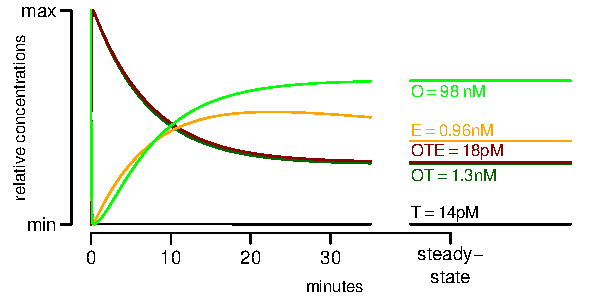
\includegraphics[width=0.75\textwidth]{Vignette2-Fig1}
\end{Ncenter}
\caption{2a: Time resolved simulation of the relative concentrations of key species}
\end{figure}

\subsection*{Figure 2b: Simulated dose-response curve}
Given a set of parameters the R-function \texttt{Trel()} from the ASOmodels package calculates the relative target concentration as a function of the total concentration of oligonucleotide added to the system.
\begin{Schunk}
\begin{Sinput}
> curve(Trel,1E-3,5E2,log='x', lwd=2,ylim=c(0,1),
+       ylab=expression(T[rel]),xaxt='n',
+       xlab='Total oligonucleotide conc (nM)')
> abline(h=Trel(1E9),lty=2) #Trel,min
> abline(v=EC50(parms['KdOT']),lty=2) #EC50
> axis(1,at=10^c(-3,-1,1,3),
+      labels=pretty10expLP(10^c(-3,-1,1,3),drop.1=T))
> axis(1,at=EC50(parms['KdOT']),label=expression(EC[50]))
> axis(2,at=Trel(1E6),
+      label=expression(T[rel*','*min]),las=1)
\end{Sinput}
\end{Schunk}
\begin{figure}[!h]
\begin{Ncenter}
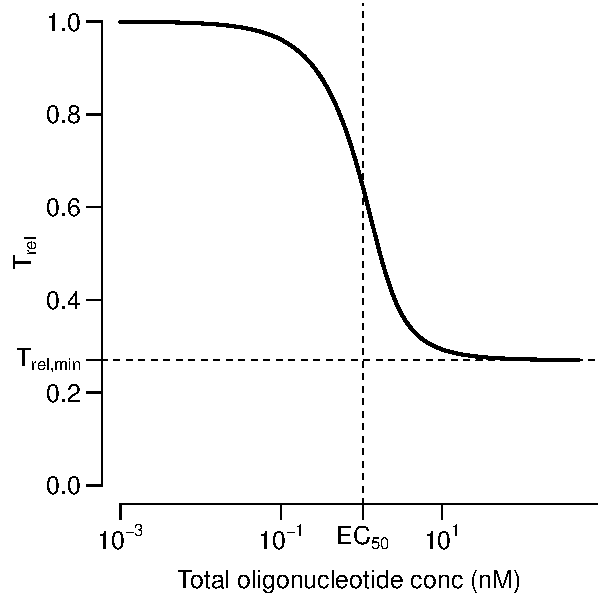
\includegraphics[width=0.5\textwidth]{Vignette2-Fig2}
\end{Ncenter}
\caption{2b: The relative total target concentration ($\Trel$) is defined as the steady state level of total target in the presence of oligonucleotide divided by the target concentration in the absence of oligonucleotide. Dashed lines indicate efficacy (horizontal) and $EC_{50}$ (vertical).}
\end{figure}


\subsection*{Figure 2c: An optimum affinity}
For a range of affinities \texttt{D1\_seq} the $EC_{50}$ values are calculated by use of the R-function \texttt{EC50()} from the ASOmodels package:
\begin{Schunk}
\begin{Sinput}
> D1_seq <- 10^seq(-3,3.2,by=0.25)
> ECfit <- sapply(D1_seq,EC50)
\end{Sinput}
\end{Schunk}
When there is no coupling between the off-rates $\kmo$ and $\kD$ then the value of $\kD$ is set in the param vector as the entry \texttt{'kC'}:
\begin{Schunk}
\begin{Sinput}
> parmsNO <- c(parms,kC=parms['kOpT']*parms['KdOT']/parms['alpha'])
> names(parmsNO)[length(parmsNO)] <- 'kC'
> ECfitNO <- sapply(D1_seq,EC50NO) #EC50 without coupling
\end{Sinput}
\end{Schunk}
For the range of affinities the corresponding $EC_{50}$-values are plotted:
\begin{Schunk}
\begin{Sinput}
> plot(D1_seq,ECfit,log='xy',yaxt='n',type='l',xaxt='n',
+      xlab=expression(K[dOT]~'(nM)'),ylab=expression(EC[50]~'(nM)'))
> lines(D1_seq,ECfitNO,lty=2)
> axis(2,at=c(2,20,200),labels=c(2,20,200),las=2)
> axis(1,at=10^pretty(log10(D1_seq)),
+      labels=pretty10expLP(10^pretty(log10(D1_seq)),drop.1=T),)
> legend('topleft',c('Coupling','No coupling'),lty=c(1,2),bty='n')
\end{Sinput}
\end{Schunk}
\begin{figure}[!h]
\begin{Ncenter}
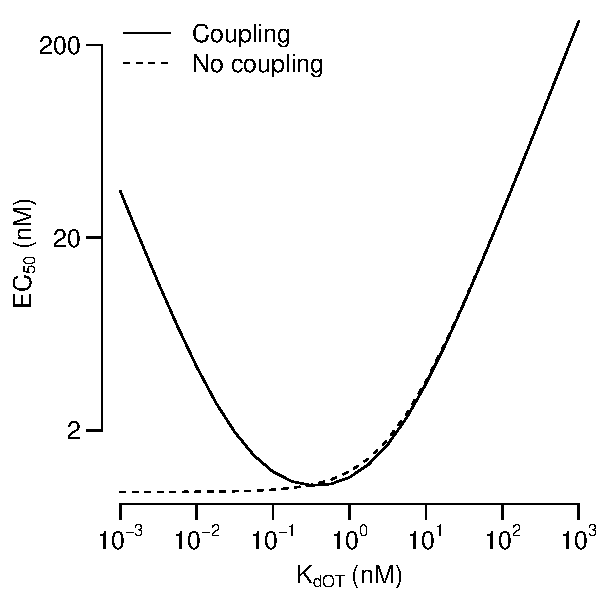
\includegraphics[width=0.5\textwidth]{Vignette2-Fig3}
\end{Ncenter}
\caption{2c: $EC_{50}$ as a function of the dissociation constant for the OT complex. A low $K_{dOT}$ corresponds to a high affinity binding. Dashed line: no coupling of off-rates. Solid line: coupling of off-rates.}
\end{figure}

\section*{Experimental data figures}
\subsection*{Figure 2d: Frieden et al. (2003)}
\begin{Schunk}
\begin{Sinput}
> data(gapmers)
> dat <- data.frame(gapmers)
> colL <- c('red','orange','darkgreen','','darkblue','','purple','','black')
> OLength <- sort(unique(dat$Oligo.length))
> #### We plot the data from Frieden et al, 2003
> dat.F <- dat[dat$Study=="Frieden 2003",]
> Flength <- dat.F$Oligo.length
> par(mar=c(4,4,1,1),las=1,bty='n',mgp=c(2.5,0.6,0))
> Fx <- dat.F$Predicted.Tm; Fy <- dat.F$Dose.2nm
> plot(Fx,Fy, pch=19, cex=2,col=colL[Flength-11],ylim=c(0,104),
+      ylab='activity (% of control)',
+      xlab=expression(T[m]~'('*degree*C*')'))
> FitF <- lm(Fy ~ Fx + I(Fx^2))
> Parfun <- function(D1){tmp <- coefficients(FitF) ;  tmp[1]+tmp[2]*D1+tmp[3]*D1^2}
> curve(Parfun(x),min(Fx),max(Fx), lwd=1,add=T,col='grey')
> f <- summary(FitF)$fstatistic
> p <- pf(f[1],f[2],f[3],lower.tail=F)
> tmp <- coefficients(FitF) ; xmin <- -tmp[2]/(2*tmp[3])
> mtext(paste('p-value =',signif(p,2)),3,line=-1)
> mtext(as.expression(substitute(Optimum~T[m] == x*degree,list(x=round(xmin)))),
+       3,line=-2.1)
> title('Luciferase')
> points(Fx,Fy,pch=19,cex=2,col=colL[Flength-11])
\end{Sinput}
\end{Schunk}
\begin{figure}[!h]
\begin{Ncenter}
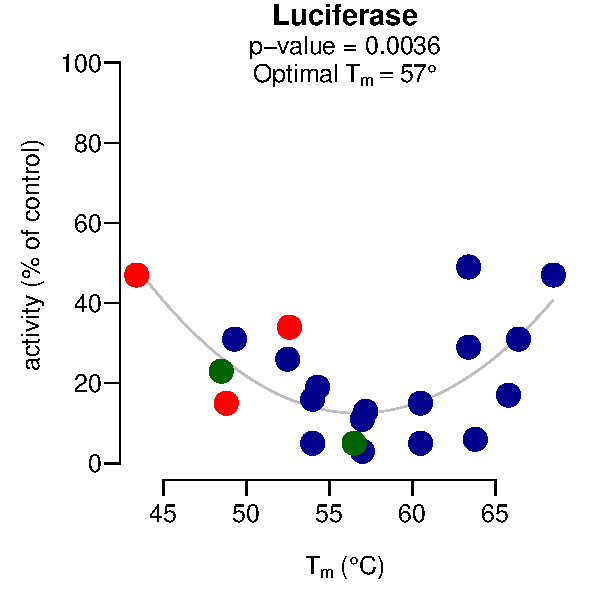
\includegraphics[width=0.5\textwidth]{Vignette2-Fig4}
\end{Ncenter}
\caption{2d:  21 oligonucleotides targeted against the luciferase firefly gene.}
\end{figure}

\section*{Figure 2e: Stanton et al. (2012)}
\begin{Schunk}
\begin{Sinput}
> #### We plot the data from Stanton et al 2012
> dat.S <- dat[dat[,1]=="Stanton 2012",]
> Slength <- dat.S$Oligo.length
> par(mar=c(4,4,1,1),las=1,bty='n',mgp=c(2.5,0.6,0))
> Sx <- dat.S$Predicted.Tm; Sy <- dat.S$Dose.3nm
> plot(Sx,Sy, pch=19,col=colL[Slength-11],ylim=c(0,104),
+      ylab='mRNA (% of control)', xlab=expression(T[m]~'('*degree*C*')'))
> legend('bottomright',as.character(sort(unique(OLength))),
+        pch=19,col=colL[sort(unique(OLength))-11],bg='white',horiz=T,bty='n')
> FitS <- lm(Sy ~ Sx + I(Sx^2))
> Parfun <- function(D1){
+   tmp <- coefficients(FitS) 
+   tmp[1]+tmp[2]*D1+tmp[3]*D1^2}
> curve(Parfun(x),min(Sx),max(Sx), lwd=1,add=T,col='grey')
> f <- summary(FitS)$fstatistic
> p <- pf(f[1],f[2],f[3],lower.tail=F)
> tmp <- coefficients(FitS) ; xmin <- -tmp[2]/(2*tmp[3])
> mtext(paste('p-value =',signif(p,2)),3,line=-1)
> mtext(as.expression(substitute(Optimum~T[m] == x*degree,list(x=round(xmin)))),
+       3,line=-2.1)
> title('GR')
> points(Sx,Sy,pch=19,cex=2,col=colL[Slength-11])
\end{Sinput}
\end{Schunk}
\begin{figure}[!h]
\begin{Ncenter}
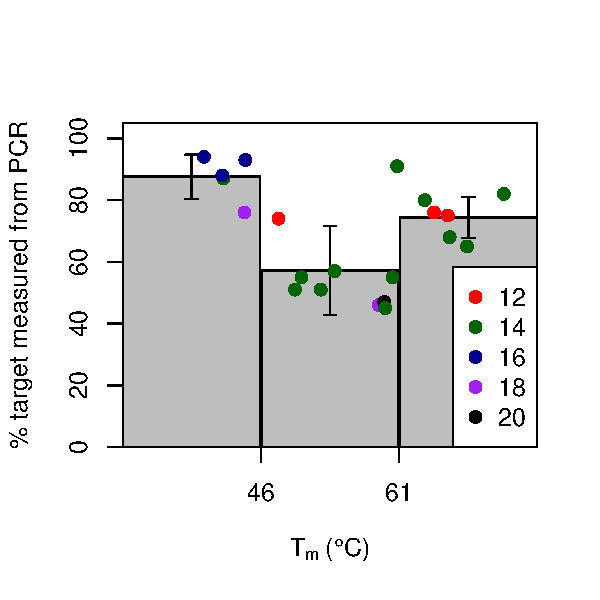
\includegraphics[width=0.5\textwidth]{Vignette2-Fig5}
\end{Ncenter}
\caption{2e: 21 oligonucleotides targeted against the glucocorticoid receptor.}
\end{figure}

\section*{Figure 2f: Pedersen et al. (2013) (this work)}
\begin{Schunk}
\begin{Sinput}
> ### We plot the data from Pedersen et al, 2013
> dat.P <- dat[dat$Study=="Pedersen 2013",]
> Plength <- dat.P$Oligo.length
> par(mar=c(4,4,1,1),las=1,bty='n',mgp=c(2.5,0.6,0))
> Px <- dat.P$Predicted.Tm; Py <- dat.P$IC50
> plot(Px,Py, xlab=expression(T[m]~'('*degree*C*')'),log='y',yaxt='n',
+      pch=19,cex=2,col=colL[Plength-11],ylab=expression(EC[50]~'('*nM*')') )
> axis(2,at=c(2E-4,1E-3,2E-3,1E-2),labels=c(0.02,0.1,0.2,1))
> FitP <- lm(log10(Py) ~ Px + I(Px^2))
> Parfun <- function(D1){tmp <- coefficients(FitP); 10^(tmp[1]+tmp[2]*D1+tmp[3]*D1^2)}
> curve(Parfun(x),min(Px),max(Px), lwd=1,add=T,col='grey')
> f <- summary(FitP)$fstatistic
> p <- pf(f[1],f[2],f[3],lower.tail=F)
> points(Px,Py,pch=19,cex=2,col=colL[Plength-11])
> tmp <- coefficients(FitP) ; xmin <- -tmp[2]/(2*tmp[3])
> mtext(paste('p-value =',signif(p,2)),3,line=-1)
> mtext(as.expression(substitute(Optimum~T[m] == x*degree,list(x=round(xmin)))),
+         3,line=-2.1)
> axis(2,1.15E-2,expression(10^-2),tick=F,mgp=c(0,-1.1,0),outer=F)
> title('APOB')
\end{Sinput}
\end{Schunk}
\begin{figure}[!h]
\begin{Ncenter}
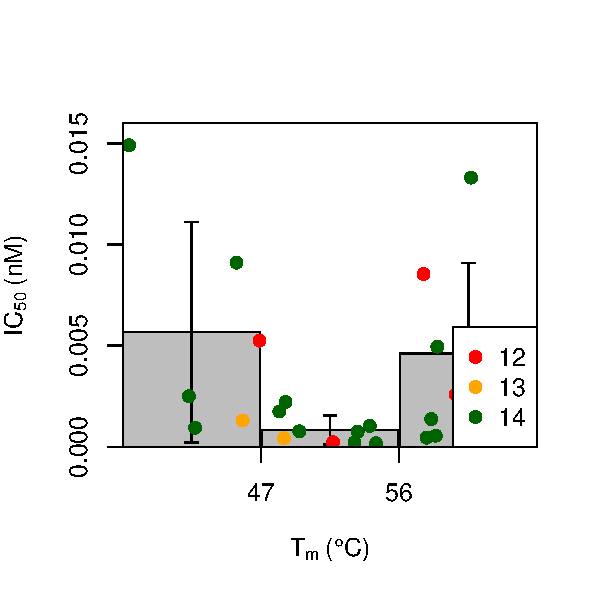
\includegraphics[width=0.5\textwidth]{Vignette2-Fig6}
\end{Ncenter}
\caption{2f: 23 oligonucleotides targeted against ApoB.}
\end{figure}


\end{document}
